
\begin{frame}
	\frametitle{Classificazione dei dati di conformance}
	\begin{figure}
	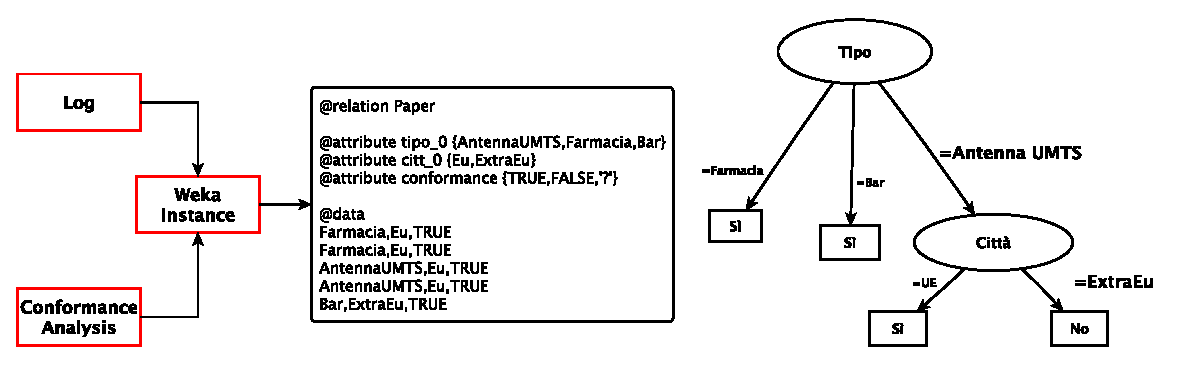
\includegraphics[scale=0.6]{./fig/decisiontree1}
	\end{figure}
	\begin{block}{}
	\begin{itemize}
	\item Alcune istanze non sono conformi al modello: es. la transizione \textit{avvia istruttoria complete} \`{e} stato eseguito due volte.
	\item Le procedure del tipo impianto due dei processi di NuovaTV non rispettano il modello.
	\end{itemize}
	\end{block}
	\end{frame}
	
%	\begin{frame}
%	\frametitle{Possibili misure correttive}
%	\begin{block}{A livello di processo}
%	Riorganizzazione del processo aziendale: giudicare ragionevole saltare le fasi di valutazione per i clienti consolidati.
%	\end{block}
%	\begin{figure}
%	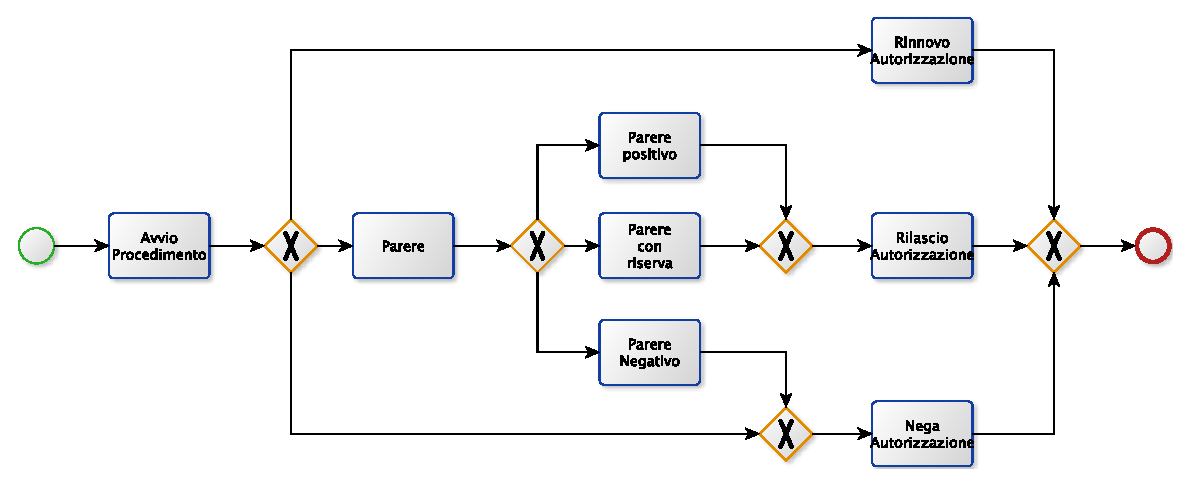
\includegraphics[scale=0.4]{./fig/BPMN}
%	\end{figure}
%	\begin{block}{Predizione}
%	Uso del classificatore in senso predittivo: prevedere i casi di non conformit\`{a} con segnalazione al personale per evitare errori noti.  
%	\end{block}
%	\end{frame}
	